\chapter{The LHC and the CMS Detector}

% **************************** Define Graphics Path **************************
\ifpdf
    \graphicspath{{Chapter3/Figs/Raster/}{Chapter3/Figs/PDF/}{Chapter3/Figs/}}
\else
    \graphicspath{{Chapter3/Figs/Vector/}{Chapter3/Figs/}}
\fi


%********************************** % First Section  *************************************
\section{The Large Hadron Collider}  %Section - 1.1 
\label{sec:detector_lhc}

The Large Hadron Collider (LHC) is a 27 km circumference proton-proton 
synchrotron accelerator with a maximum design centre of mass energy,
$\sqrt{s} = 14$ \tev. It is the highest energy component of the CERN accelerator
complex (figure~REF). The LHC accelerates counter-rotating beams of protons 
using 400 MHz radio frequency
(RF) cavities, focusses the beam using multiple quadrupole and higher order magnets,
and maintains the beams trajectory using super-conducting, niobium-titanium 
dipole magnets, capable of producing an 8.4 Tesla magnetic field. This high 
magnetic field is achieved by cooling the magnets to 1.9 K using super-fluid 
helium, and applying a 11.85 kA electric current.

The beams, consisting of approximately 1400 bunches of $~1.1x10^{11}$ protons,
are brought into collision
at four points around the LHC ring within specialised detector systems. During the
first run of the LHC, `Run I', bunches were spaced in 50 ns intervals, leading to
a bunch crossing rate of 20 MHz. Collisions continue for a number of hours, 
while collision rates are maintained by scanning the transverse beam positions, 
until such a time when proton numbers are depleted, the beam is dumped and the 
fill process repeated.

Simultaneous interactions happening at the time
of each bunch crossing are referred to as in-time pile up (PU), 
causing experimental challenges for detector readout and event reconstruction.

\emph{instantaneous and integrated luminosity}

The four detectors of the LHC consist of \texttt{ALICE}, \texttt{ATLAS},
\texttt{CMS} and \texttt{LHCb}. Of these, both \texttt{ATLAS} and \texttt{CMS} 
are considered as general purpose detectors, optimised for the investigation of
high-\Pt phenomena, making them ideal detectors for new physics.

The work in this thesis uses the \texttt{CMS} detector, which is discussed in 
the following section.


%********************************** % Second Section  *************************************
\section{Compact Muon Solenoid}  %Section - 1.2 
\label{sec:detector_overview}

CMS, standing for `Compact Muon Solenoid' (figure~\ref{fig:cms_diagram}), is a
hermetic detector system 
optimised for the study on high-\Pt objects and their decays, produced in the 
proton collisions at the LHC. It is designed to make accurate measurements of 
the positions and momenta of physics objects such as electrons, muons, taus, 
photons and jets. Owing to an almost complete 4$\pi$ solid angle coverage, CMS is 
capable of also making accurate measurements of global energy imbalances due to 
the presence of weakly interacting particles.

\begin{figure}[hb!]
  \centering
  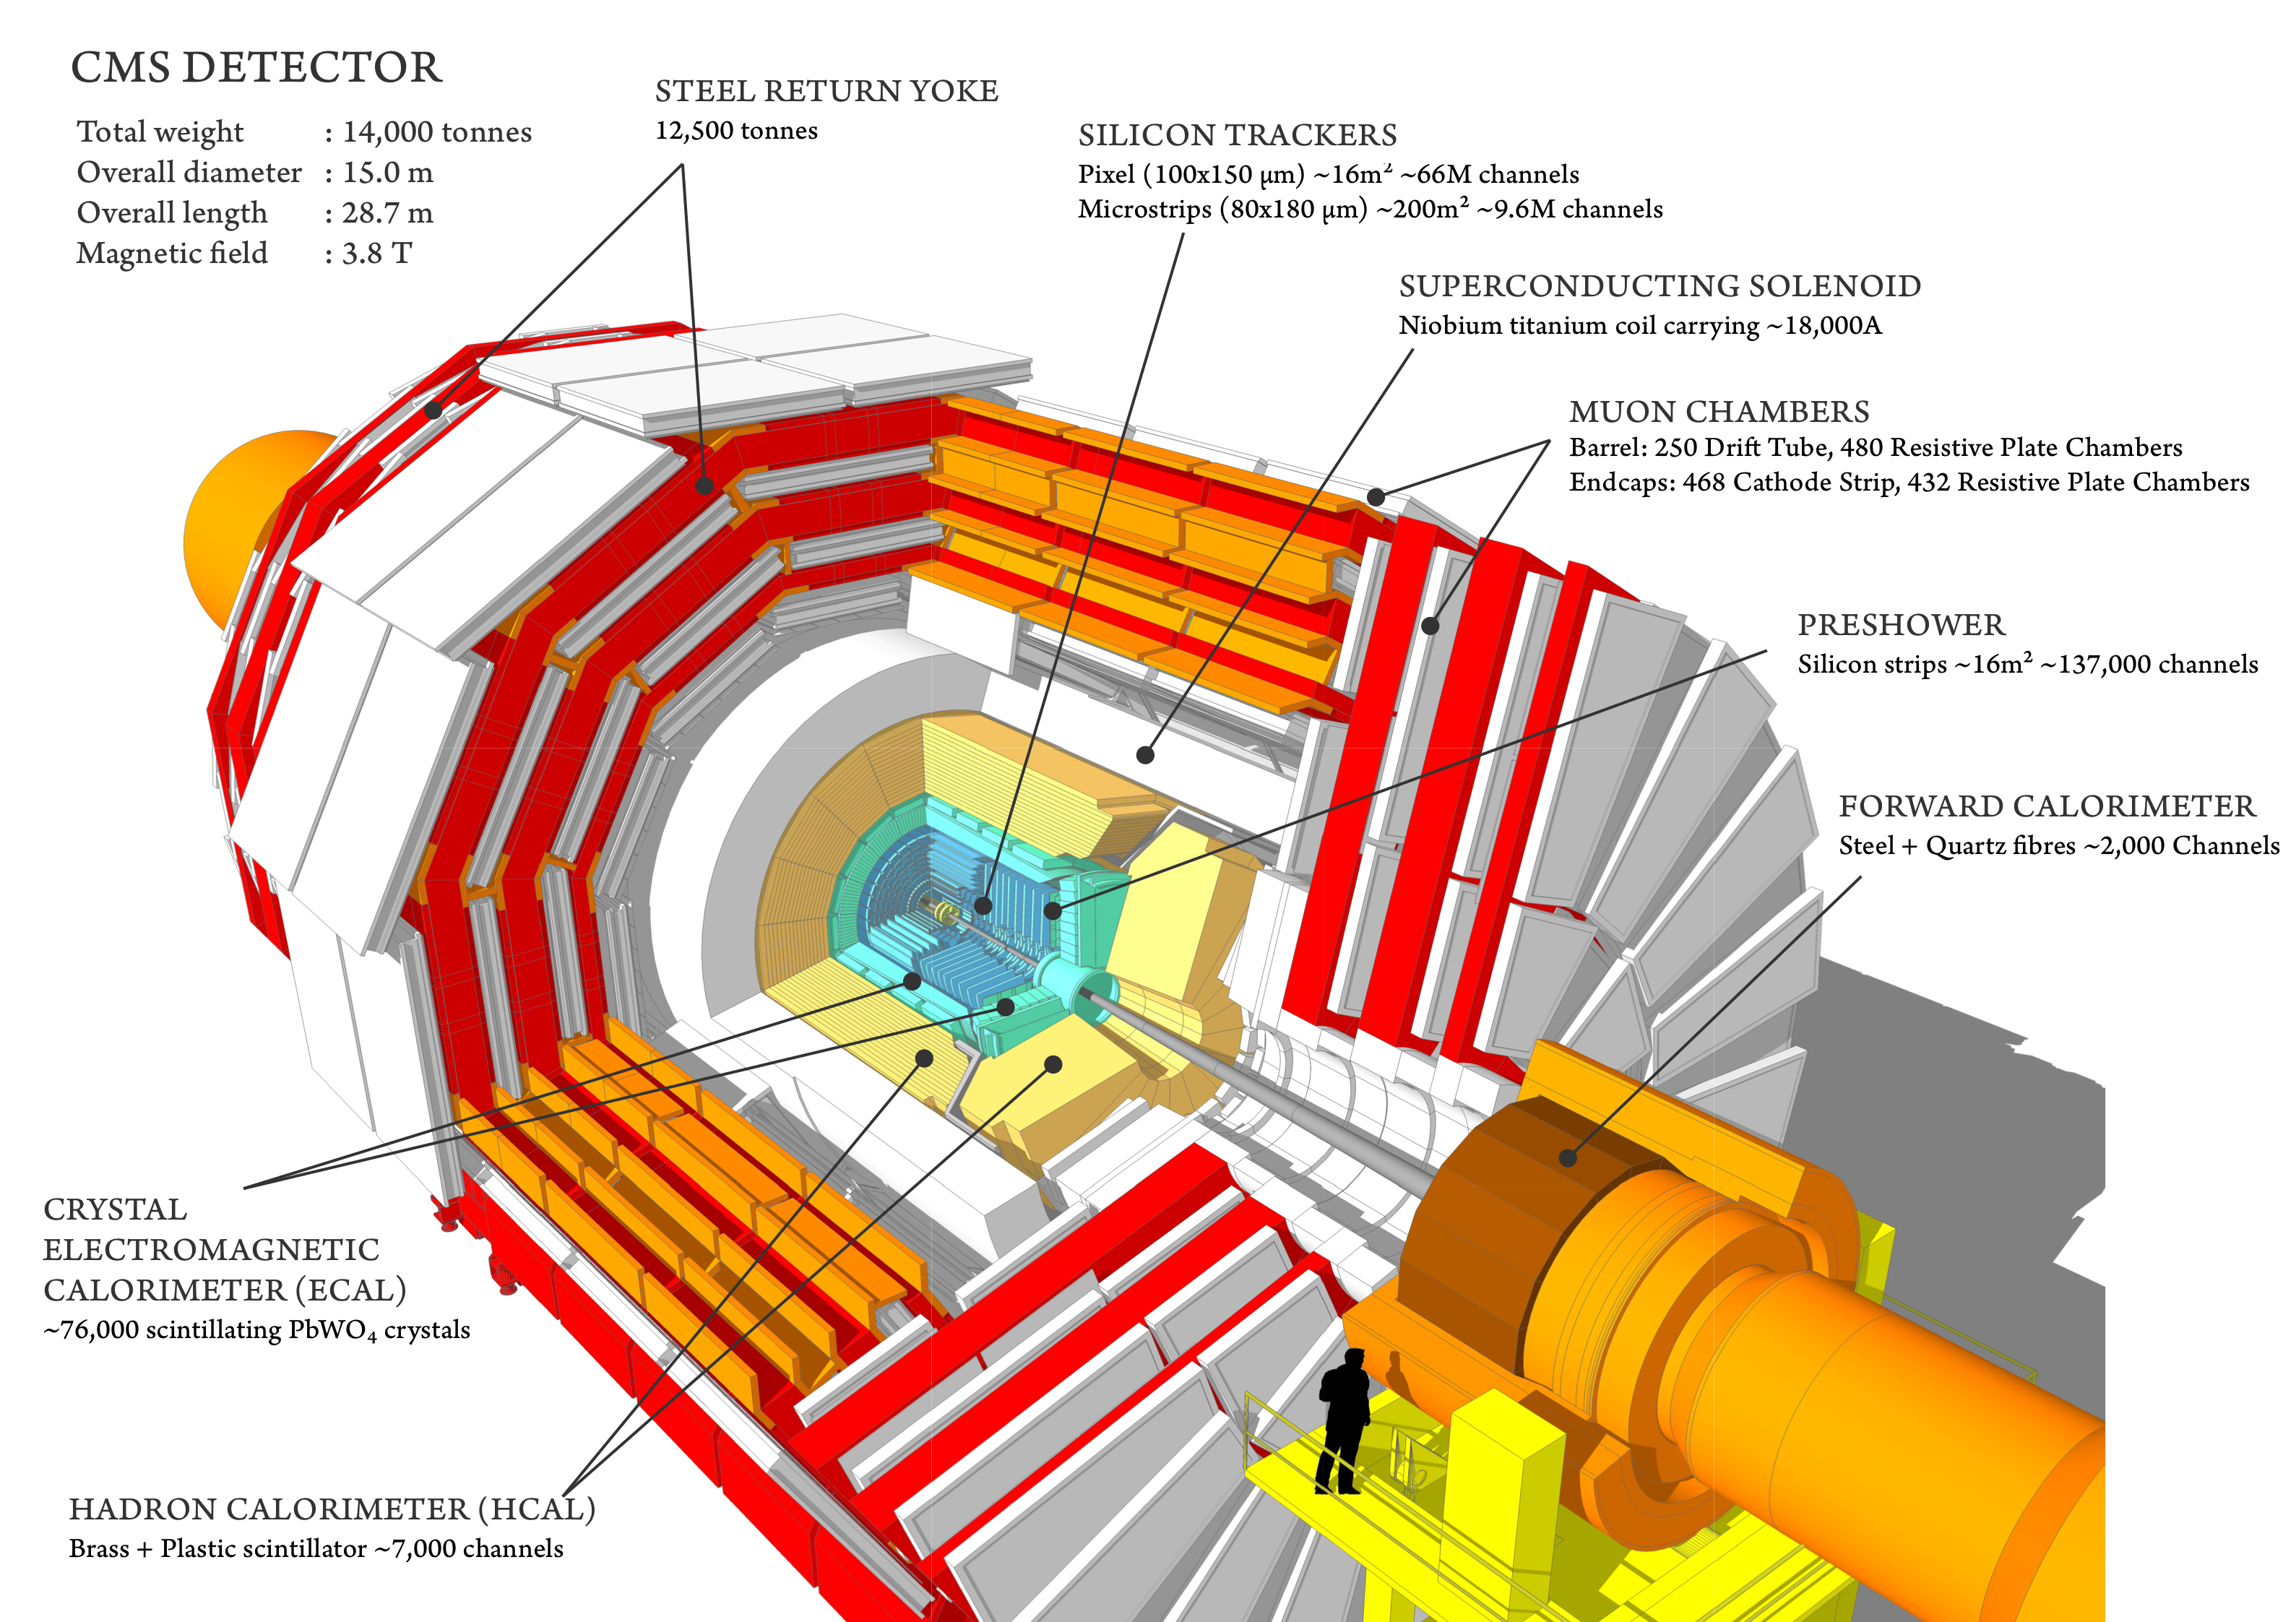
\includegraphics[width=\textwidth]{Figs/cms_120918_02.png}
  \caption{Diagram of the Compact Muon Solenoid REF.}
  \label{fig:cms_diagram}
\end{figure}

The cylindrical detector is 28 m in length, 15 m in diameter and has a mass of 
around 14,000 tonnes \footnote{if it was placed in the bath, it would sink.}. 
The z-axis is taken to be the longitudinal dimension along the beamline, the x-
axis the perpendicular direction pointing towards the centre of the LHC ring, 
and the y-axis pointing skywards, perpendicular to these forming a right-handed 
co-ordinate system. The transverse plane is taken to be the plane of the x and y
axes.

Directions relative to the CMS detector are described with the variables $\phi$,
the angular direction in the transverse plane with the range $[-\pi, \pi]$, and 
the pseudo-rapidity, $\eta$, describing the angle with respect to the z-axis,
defined as:

\begin{equation}
\eta = - ln \Bigg[ tan \Bigg( \frac{\theta}{2} \Bigg) \Bigg]
\end{equation}

where blah blah. Differences in these two variables, $\Delta \phi$ and $\Delta 
\eta$, are invariant under Lorentz boosts, and so can be used to construct a 
furthermore Lorentz-invariant angular separation between particles:

\begin{equation}
\Delta R = \sqrt{ (\Delta \eta)^2 + (\Delta \phi)^2}
\end{equation}

CMS is arranged in a layered configuration of sub-detectors, structured as a 
cylindrical barrel, `closed' by two end-caps. The barrel contains a
super-conducting solenoid magnet capable of producing a 3.8 T magnetic field. 
Operated at 4.5 K, with a 18.5 kA current, the longitudinal field produced bends
the trajectories of charged particles allowing for precise charge and momenta 
measurements.

%********************************** % Third Section  *************************************
\section{Detector Subsystems}  %Section - 1.3
\label{sec:detector_subsystems}

Detector subsystems within CMS follow a layered structure in both the barrel and
end-cap regions. The following describe each of the subsystems in more detail.

\subsection{Tracker}
% - inner three layers of pixel detectors
%     - also have end-caps of pixel detectors
% - what type of pixels? what pitch? technology?
% - provide 2d information of hit positions

% - further 10 layers of silicon strip detectors
%     - n-in-p?
%     - and end-

% - this detector system provides information of not only the vertex location and 
% tracking of charged particles, but also given the massive magnet, a 
% determination of both their charge and momenta.

The silicon tracker system consists of an inner pixel-based and outer strip-
based detectors.

The pixel detector consists of three layers of silicon pixel sensors situated 
as close as 4 cm from the beamline, capable 
of producing 2D hit information of charged particles for use in vertex 
finding. The barrel section is also accompanied by two end-cap pixel detector 
disks. Each sensor contains a 52 x 80 grid of 100 \microm x 150 \microm pixels, 
and are mounted on a lightweight mechanical substrate along with front-end readout 
electronics.

A further 10 layers of silicon strip detectors are used to accurately 
reconstruct the track path of charged particles. The sensors collectively cover 
an area of over 200 $\text{m}^2$, are of p-in-n type, and range from 320 \microm
to 500 \microm in thickness and pixel pitch ranging between 80 \microm and 
205 \microm, depending on distance from the beamline.

All silicon detectors situated so close to the interaction point receive high-
doses of radiation, eventually ageing due to the damage inflicted. Subsequently, 
radiation hard sensor and front-end electronics designs have been carefully 
selected to mitigate the effects of ageing due to radiation damage.

\subsection{Electromagenetic Calorimeter}

% - ecal made of scintillating lead tungstate (PbWO4) crystals
%     - each crystal is 0.017 x 0.017 (in deltaEta x deltaPhi dimensions), and 23 
%     cm in length
%         -   corresponds to about 25 radition lengths
%         - moliere radius?
%     - super-crystal arrangement?
% - each crystal has a photodetector to determine the level of scintillation light
% produced
%     - avalanche photo-diodes in the barrel, and vacuum photo-triodes in the 
%     endcap region
%     - radiation hardness?
%     - what material?

% - this detector system provides energy and spatial information of
% electromagnetically showering particles.

The Electromagnetic Calorimeter (ECAL) system provides accurate measurements of 
energy deposits of electromagnetically interacting particles such as 
electrons and photons. The detector consists of scintillating lead-tungstate
($\text{PbWO}_4$) crystals, each of dimension 0.017 x 0.017 ($\Delta \eta \times
\Delta \phi$) and 23 cm in length, corresponding to around 26 radiation length 
and providing a Moli\`'{e}re radius of 2.2 cm. In both the barrel and the
end-cap regions, individual crystals are clustered
into super-towers, to match with towers in the trigger system
(the calorimeter trigger system is described later in
section~\ref{sec:detector_trigger}).

Scintillation light produced in each crystal is collected by a photo-detector - 
avalanche photo-diodes in the barrel and vacuum photo-triodes in the endcap. The
detectors are required to be both radiation hard and capable of operating within
the strong magnetic environment of CMS.

The ECAL determines precise measurements of the energies and identification of
particles, and can also produce spatial measurements when used in conjunction 
with data from the tracker system.

\emph{can i ignore the pre-shower rubbish, as we don't consider endcap objects? 
- or do we for electromagnetic particles?!}

\subsection{Hadronic Calorimeter}

% - alternating layers of brass absorber and plastic scintillator
% - scintillators are sectioned into towers, 0.087x0.087 in barrel and 0.17x0.17 
% in the endcaps (double check this isn't just my interpretation of ted's eta 
% numbers)
% - light produced in the scintillator layers is transmitted via wavelength 
% shifting fibres to a hybrid photo-diode for detection

The Hadronic Calorimeter (HCAL) system measures the energy of hadronic showers 
originating from single-quarks and gluons (i.e. jets). It is constructed from
alternating  brass absorber and plastic scintillator layers. The latter are spatially 
segmented into towers measuring 0.087 x 0.087 and 0.17 x 0.17 in the barrel and 
end-caps respectively (CHECK DIMENSIONS). Hadronic showers of particles deposit 
energy as scintillation light in the plastic layers, which is transmitted via 
wavelength shifting fibres to be measured in hybrid photo-diodes. 

\emph{can i ignore the HF region, as we ignore forward jets?}

\subsection{Muon Systems}

% - comprised of three different gaseous detector technologies, each with 
% different coverages in eta
% - drift tubes (DT)
%   - traditional technology, optimised for low occupancy
%   - central: eta < 1.2
% - cathode strip chambers (CSC)
%   - designed for high magnetic field and neutron backgrounds
%   - forward: 0.9 < eta < 2.4
% - resistive plate chambers (RPC)
%   - designed for high magnetic field and neutron backgrounds
%   - forward and central eta < 2.1

Muons are detector in the outer layers of the detector, with the muon system 
comprised of three different gaseous detector technologies each with different 
pseudo-rapidity coverages. The central region, $|\eta|<1.2$ is equipped with 
Drift Tube (DT) detectors - a traditional detector technology, optimised for low
-occupancy measurements. Cathode Strip Chambers (CSC) cover the forward region,
$0.9 < |\eta| < 2.4$, and dual-layered Resistive Plate Chambers (RPC) cover
$|\eta| < 2.1$ - both CSC and RPC detectors being optimised for operation in 
both high magnetic field and neutron background environments.

The muon system aims to provide identification and precision measurements of
muon momenta. Energy deposits in the muon systems can be combined with 
information from the tracker to improve momentum resolution significantly.

%********************************** % Fourth Section  *************************************
\section{Trigger and Data Acquisition}  %Section - 1.4
\label{sec:detector_trigger}

\subsection{Trigger system}
Events of interest are selected using a dedicated triggering system. It is 
split into two distinct stages: the hardware-based Level 1 (L1) and
the software-based High-Level Trigger (HLT) systems.

\subsubsection{Level-1 Hardware Trigger}
% - L1 system is hardware based running at a rate of 40 MHz
% - runs on coarse trigger primitive objects, constructed from raw energy deposits
% in the calorimeter and muon systems independently
%     - takes regional information from both the calorimeter and muon systems 
%     independently.
%     - combines regional data in the GCT/GMT
%     - feeds combined objects (from across entire detector) into the GT, where a 
%     L1 accept is made or not.
% \emph{can talk in more detail here about the calorimeter trigger path and the 
% GCT's job}
% - has approximately 3microsecs per events
% - objects considered at L1 are electrons, muons, jets (central and forward) and 
% energy sums (ETT, MET, HTT, MHT)
% - L1Accept is made dependent on the objects within an event meeting 1 of 127 (
% check!) simple threshold and multiplicity based requirements.
% - maximum available output bandwidth of the L1 system is 100 kHz, although the 
% output rate is kept lower than this to allow for stochastic fluctuations

The L1 system consists of a staged, modular design of custom built hardware 
electronics systems, shown in figure~\ref{fig:l1_diagram}. 
The L1 trigger reconstructs energy deposits in the calorimeters and muon systems
into coarse `trigger-primitive' physics objects, in the calorimeter and the muon 
trigger respectively. Regional information is gathered by separate modules 
before being combined in the Global Calorimeter Trigger (GCT) and Global Muon 
Trigger (GMT) systems, where physics objects are sorted according to energy. 
Finally, an event's objects are passed on to the Global Trigger (GT) where a 
`Level-1 Accept' (L1A) signal is issued or not, dependent on the event meeting 
one of 127 (CHECK) simple object threshold and multiplicity based requirements.

\begin{figure}[ht!]
  \centering
  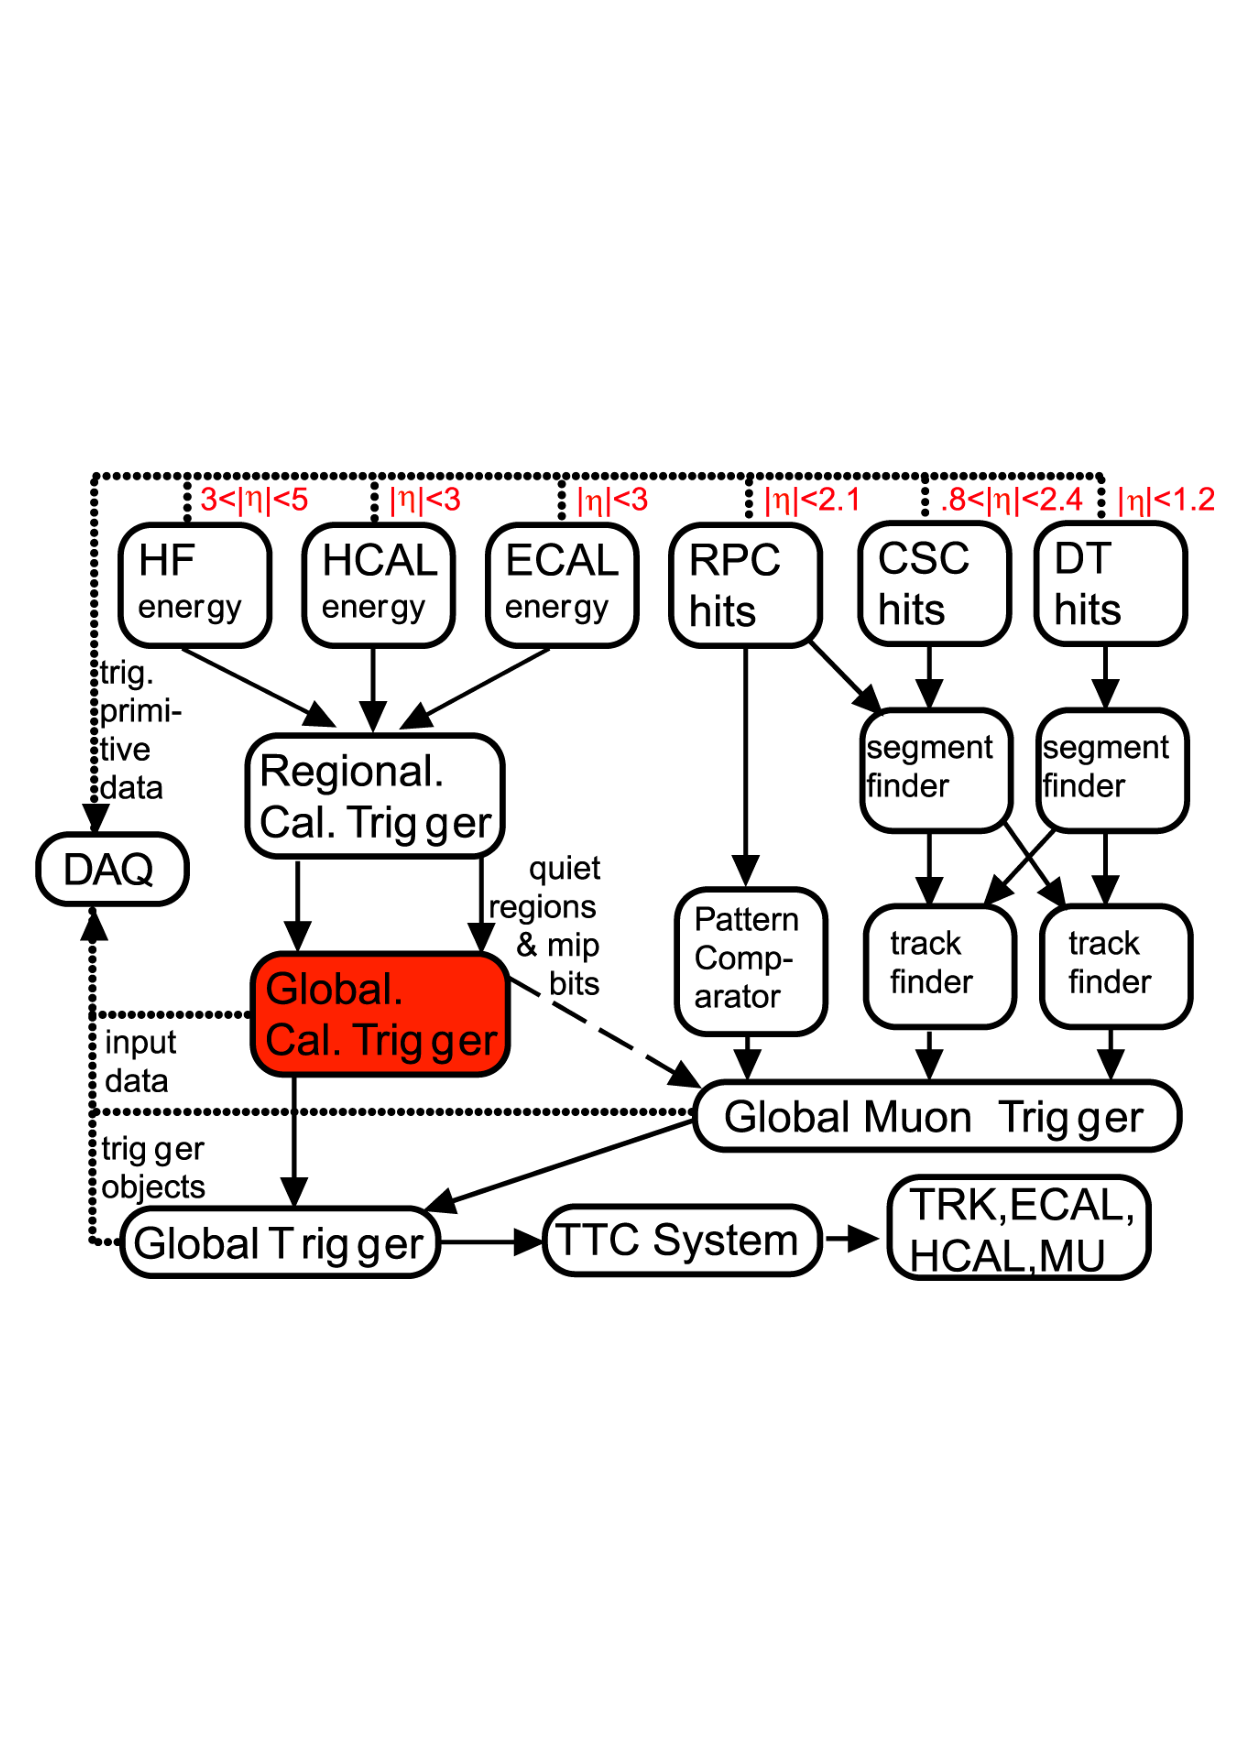
\includegraphics[width = 0.7\textwidth]{Figs/trigger/L1_diagram.pdf}
  \label{fig:l1_diagram}
  \caption{Schematic overview of the Level-1 hardware trigger system of CMS.}
\end{figure}

The L1 system is required to run at 40 MHz, equal to the maximal bunch-crossing
rate within CMS, with a L1A decision required within a latency of 3 $\mu s$. The
maximum available output bandwidth is 100 kHz, but is typically maintained at a 
lower value to allow for stochastic fluctuations in rate.

\subsubsection{High-level Trigger}
% - Following a L1A signal, candidate events are optically transmitted to the high
% level trigger, consisting of a large computer farm of the off the shelf server 
% PCs
% - events are reconstructed/built in more detail
% - passed on to a suite of analyst-designed software triggers which can 
% reconstruct more advanced objects and event variables, such as alphaT (as 
% described later in chapter BLAH) - has approximately 50ms per event
% - HLT reduces rate to around 300 events per second

Following a L1A signal, candidate events are optically transmitted to the HLT 
system, consisting of a large computer farm of the off the shelf server 
PCs. Events are reconstructed in greater detail, due to the increase in 
processing time of up to 50 ms, allowing for a closer emulation of offline 
reconstruction techniques. Complex analyst-designed trigger rules are used, 
which can employ more sophisticated event-level variables such as \alphat
(described in detail later in chapter~\ref{ch:5}).

The HLT reduces event rates further by around two orders of magnitude, typically
outputting hundreds of events per second. Events passing the HLT are transmitted
on for full offline reconstruction.
